\documentclass[12pt, openany]{report}
\usepackage[utf8]{inputenc}
\usepackage[T1]{fontenc}
\usepackage[a4paper,left=2cm,right=2cm,top=2cm,bottom=2cm]{geometry}
\usepackage[frenchb]{babel}
\usepackage[pdftex]{graphicx}
\usepackage{amsmath,amsfonts,amssymb}
\usepackage{hyperref}
\usepackage{color}
\usepackage[table]{xcolor}
\usepackage{listings}
\usepackage{enumitem}
\usepackage{pifont}
\usepackage{ragged2e}
\usepackage{tabto}


\setlength{\parindent}{0cm}
\setlength{\parskip}{1ex plus 0.5ex minus 0.2ex}
\newcommand{\hsp}{\hspace{20pt}}
\newcommand{\HRule}{\rule{\linewidth}{0.5mm}}
%\renewcommand{\thesection}{\Roman{section}}
\renewcommand{\thesection}{\arabic{section}} 
\setcounter{secnumdepth}{4}
\setcounter{tocdepth}{4}

%contenu du document
\begin{document}


\begin{titlepage}
  \begin{sffamily}
  \begin{center}
	
\includegraphics[scale=0.5]{ub.png}~\\[1cm]

    \textsc{\Large MASTER 2 Informatique RCI }\\[1.5cm]
    2021-2022

    % Titre
    \rule{1\linewidth}{2pt}
     \\[1cm]
    { \huge \bfseries Rapport de PFE :\\
    Déploiement d'un VPN sur des équipements mobiles ou IoT\\[1cm] }
    \rule{1\linewidth}{2pt}
    \\[1cm]
    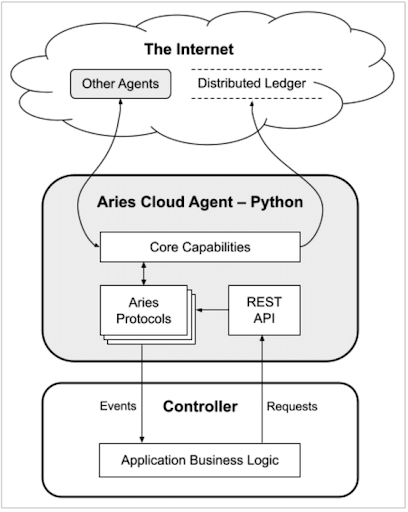
\includegraphics[scale=0.55]{couv.png}
    \\ %[1cm]

    % Membres du groupe
   \vfill
      \begin{center}
        %\hspace*{3.1cm}
        \Large	 Alexis Henquinet \hspace*{1cm} Mohamed Diallo \hspace*{1cm} Sara Real Santos
      \end{center}
 
    % Bas de la page
 
  \end{center}
  \end{sffamily}
\end{titlepage}

\newpage

\renewcommand{\contentsname}{Sommaire}
%\addcontentsline{toc}{section}{Remerciements}
\tableofcontents
\newpage

\section{Introduction}
\subsection{Contexte}
\noindent 
\begin{flushleft}
De nos jours l'emploi de réseaux privés virtuels (VPN, Virtual Private Network) est de plus en plus démocratisé. On s'en sert généralement pour masquer son adresse ip, ou pour créer un canal sécurisé chiffré avec un destinataire. De nombreuses applications, services et protocoles de VPN différents existent, que ce soit sur Ordinateur ou Smartphone.\\
En tant qu'utilisateur, se connecter à un serveur VPN nécessite d'en connaitre son adresse ip ainsi qu'échanger des clés de chiffrement (symétrique ou asymétriques) avec celui-ci. Cependant pour garantir l'authenticité de la connexion, et identifier le serveur/client avec lequel le tunnel VPN s'établit, on peut recourir aux Certificats. Lorsqu'un client veut se connecter à un serveur, il lui demande son certificat afin de prouver son identité. Ce certificat étant délivré par un tier de confiance, à savoir l'Autorité de certification, le client peut donc avoir une preuve de l'identité du serveur. Cependant, ce système étant centralisé, il dépend des autorités de certification et peut présenter différents problèmes. D'une part la possible censure ou contrôle de la part de cette autorité, mais aussi le fait que si jamais cette autorité est attaquée, alors tous les certificats délivrés par celle-ci sont compromis. Pour pouvoir contrer ces difficultés, de nouvelles méthodes basée sur la décentralisation des autorités de certifications existent, comme par exemple basées sur la BlockChain.\\
\end{flushleft}

\subsection{Présentation du projet}
\noindent 
\begin{flushleft}
\textit{Déploiement d'un VPN sur des équipement mobiles ou IoT} est un projet dont le but est de réussir à installer et configurer le VPN WireGuard sur un client Android. Cet Android sera une machine virtuelle qui s'appuie sur les logiciels QEMU et KVM, et membre d'un réseau virtuel NEmu.\\
WireGuard est un VPN nécessitant des couples de clés publique/privée de chiffrement asymétrique. Afin de garantir l'authentification et l'identité du serveur VPN WireGuard auquel le client Android se connectera, cela nécessitera l'emploi de Verifiable Credentials (VC), un équivalent des Certificats mais dont l'autorité de certification repose sur la décentralisation, à savoir un noeud de blockchain déjà existant. Le projet Aries Hyperledger soutenu par la fondation Linux permet de développer des mécanismes basés sur les VCs. Nous utiliserons donc Aries Mobile Agent sur le client Android pour communiquer avec un Aries Cloud Agent relié à un réseau Hyperledger Indy dont le rôle est de délivrer les VC. Nous utiliserons également un Aries Cloud Agent sur le serveur WireGuard afin de communiquer avec le noeud Indy et récupérer un VC.
\end{flushleft}

\newpage
\section{Étude de l'existant}

\subsection{Wireguard}
\noindent 
\begin{center}

\includegraphics[width=\textwidth]{wg.png}
\end{center}

\begin{flushleft}
WireGuard est un VPN fonctionnant sur la couche 3 du modèle OSI. Il est implémenté comme une interface réseau virtuelle du noyau pour Linux. Il est pensé pour remplacer les VPN IPsec et ceux basés sur TLS comme OpenVPN, tout en se voulant plus sûr, performant et facile d'utilisation de part son implémentation en moins de 4000 lignes de code facilement compréhensibles et vérifiables sur les systèmes Linux.\\
Il a été initialement déployé pour les systèmes Linux, mais il dispose maintenant de portages sous Android, Windows ou macOS principalement. Pour un client, WireGuard ne nécessite qu'un échange de clés publiques et d'informations de connexions comme l'adresse ip du serveur hôte. De courtes clés statiques pré-partagées en Curve25519 (basé sur Diffie-Hellman) sont utilisées pour l'authentification mutuelle. Le protocole proposé assure une confidentialité forte ainsi qu'un haut degré de dissimulation d'identité. Au niveau du transport, il utilise le cryptage authentifié ChaCha20Poly1305 pour l'encapsulation des paquets en UDP.  La clé publique construite avec Curve25519 est utilisée pour créer une interface réseau qui lui est associée. Ces interfaces font partie de la 'cryptokey routing table', qui peut être configuré et à laquelle on peut ajouter des règles de routage supplémentaires. Quand des paquets sont envoyés vers une machine par un tunnel Wireguard (donc, par l'interface dans la cryptokey routing table), ils sont chiffrés avec la clé publique de la machine qui reçoit le paquet.\\
Il est cependant à noter que les couples de clés asymétriques publiques/privées génrérées par WireGuard à l'aide de son algorithme ne sont pas adaptables aux Certificats X509 de part leur format (32 caractères 64 bits).\\
Nous utiliserons pour notre projet la version mobile Android de WireGuard côté client, ainsi que la version Linux de WireGuard côté serveur.

\end{flushleft}

\subsection{Verifiable Credentials}
\noindent 
\begin{flushleft}
Un "credential" correspond à une accréditation, un certificat ou une référence. Par exemple dans le monde physique cela peut être une pièce d'identité, un passeport, un permis ou encore un diplôme universitaire. Avec l'avènement de la BlockChain, il est maintenant possible de représenter numériquement et de manière sûre un credential. On parle alors de Verifiable Credential, car grâce à la BlockChain il est possible de les vérifier facilement et rapidement. En Novembre 2019 le W3C a entammé une procédure de normalisation en publiant une recommandation sur les Verifiable Credentials, dans le but de garantir un format générique reconnu mondialement. Il s'agit donc d'une technologie novatrice et en pleine construction.\\
Il y est stipulé qu'un détenteur (ou "Holder") de VC peut générer une présentation à partager à quelqu'un voulant une preuve d'accréditation selon certaines caractéristiques, et ce sans forcément transmettre l'entièreté des caractéristiques de son VC. Par exemple pour obtenir un service nécessitant d'être majeur, une preuve de notre âge peut nous être demandée. Il n'est alors pas obligatoire de transmettre le champ de son VC d'identité contenant sa date de naissance, mais par exemple juste prouver dans la présentation que l'on a "plus de 18 ans".\\

Pour mieux comprendre les différents rôles et informations concernant les VCs, voici ci-dessous le schéma proposé par la W3C :\\
\begin{center}
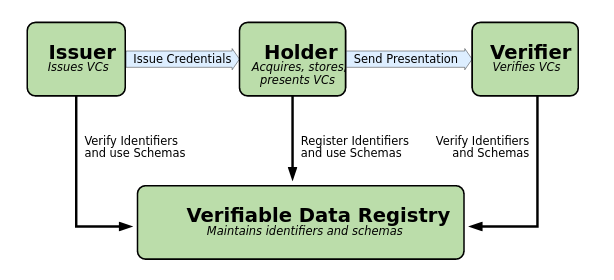
\includegraphics[scale=0.5]{vc.png}
\end{center}

Des mécanismes de preuves et de signatures numériques sont nécessaires afin d'assurer la protection d'un Verifiable Credential. L'obtention de la validation des preuves peut dépendre de la syntaxe de la preuve, cependant dans le cadre de ce projet les VCs correspondront à des JSON Web Tokens sécurisés par l'utilisation de JSON Web Signatures. Voici ci-dessous un exemple de de VC JWT présenté par le W3C :\\
\begin{center}
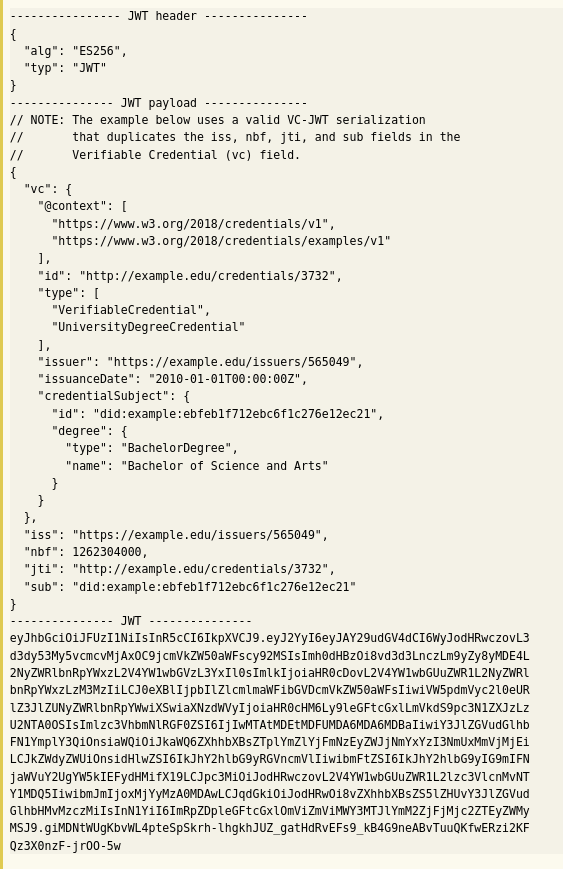
\includegraphics[scale=0.4]{vc2.png}
\end{center}
\end{flushleft}

\newpage
\subsection{Aries Hyperledger}
\noindent 
\begin{flushleft}
Aries Hyperledger est un projet developpé par l'Hyperledger Foundation. Hyperledger Foundation est une communauté centrée sur le développement d'outils, librairies et frameworks permettant de déployer des blockchains qui seront majoritairement mises au service d'entreprises. \\
Il y a différents projets lancées par la Fondation Hyperledger. Aries Hyerledger est le 13ème projet lancé par cette communauté. Aries Hyperedger est une infrastructure permettant l'échange de données en relation à la blockchain ainsi que l'échange de messages peer-to-peer. \\
\vspace{2mm}
Aries Hyperledger inclut plusieurs services dans son infrastructure :
\begin{itemize}
\item Une couche interface appelée resolver qui permet de créer et signer des transactions blockchain
\item Un wallet sécurisé permettant de garder des secrets et autres informations 
\item Un système de messagerie encrypté pour l'échange entre clients hors blockchain
\item Une implementation des W3C Verifiable Credentials 
\item Une implementation du Decentralized Key Management System (DKMS)
\item Un mechanisme qui permet de construire protocoles et des API

\end{itemize}
\begin{center}
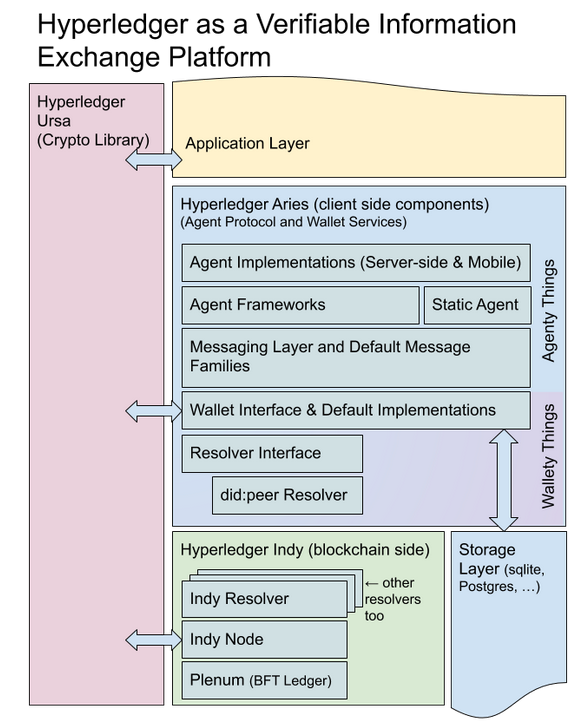
\includegraphics[scale=0.4]{aries-hyper.png}
\end{center}

\vspace{5mm}
Le plus grand objectif du projet Aries Hyperledger est de pouvoir offrir une infrastructure qui peut travailler et s'adapter à d'autres technologies développées par Indy ou qui se servent d'autres technologies blockchain. 
\end{flushleft}

\newpage
\subsubsection{Aries Cloud Agent}
\noindent 
\begin{flushleft}
Hyperledger Aries Cloud Agent Python (ACA-Py) est une projet visé à servir de base pour contruire des agent pouvant utiliser des Verifiable Credentials. Ses protocols et fonctionnalités de base permettent de délivrer, vérifier et stocker des Verifiable Credentials. Les agent ACA-Py peuvent contrôler des Verifiable Credentials de format Hyperledger Indy AnonCreds et de format W3C, dans ce projet nous nous intéréssons eu dernier format. \\
Aries Cloud Agent fonctionne avec des requêtes HTTP et des notifications webhook. Ceci ouvre la possibilité d'écrire un controlleur qui 'discute' avec notre agent en n'importe quel langage pouvant gérer des requêtes HTTP. \\
L'Agent Aries Cloud met aussi en oeuvre une interface  OpenAPI REST pouvant servir à comprendre comment les protocols dans notre agent fonctionnent. Le controller peut donc utiliser ceci pour gérer le comportement de l'agent. Voici un résume de l'architecture de l'agent Aries Cloud : \\

\begin{center}
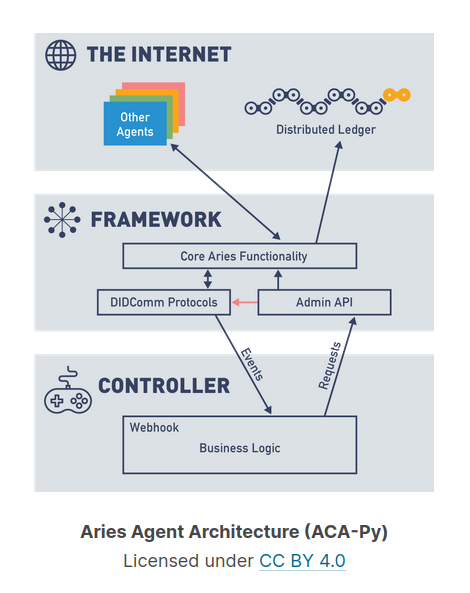
\includegraphics[scale=0.6]{ACA-py.png}
\end{center}
\end{flushleft}

\vspace{5mm}
Dans notre architecture, nous pouvons voir que notre Agent communique avec un Distributed Ledger, donc un Blockchain. Pour précision, dans notre projet nous utilisons Von Network comme Blockchain.

\vspace{2mm}
Pour controler et faire des actions dans l'API il suffit juste de retrouver le endpoint qui fera l'action qu'on veut, le sélectionner et rentrer les champs nécessaires s'il en faut. C'est un outil très outil pour comprendre et développer son agent. \\
Voici l'API d'un agent Aries Cloud : 

\begin{center}
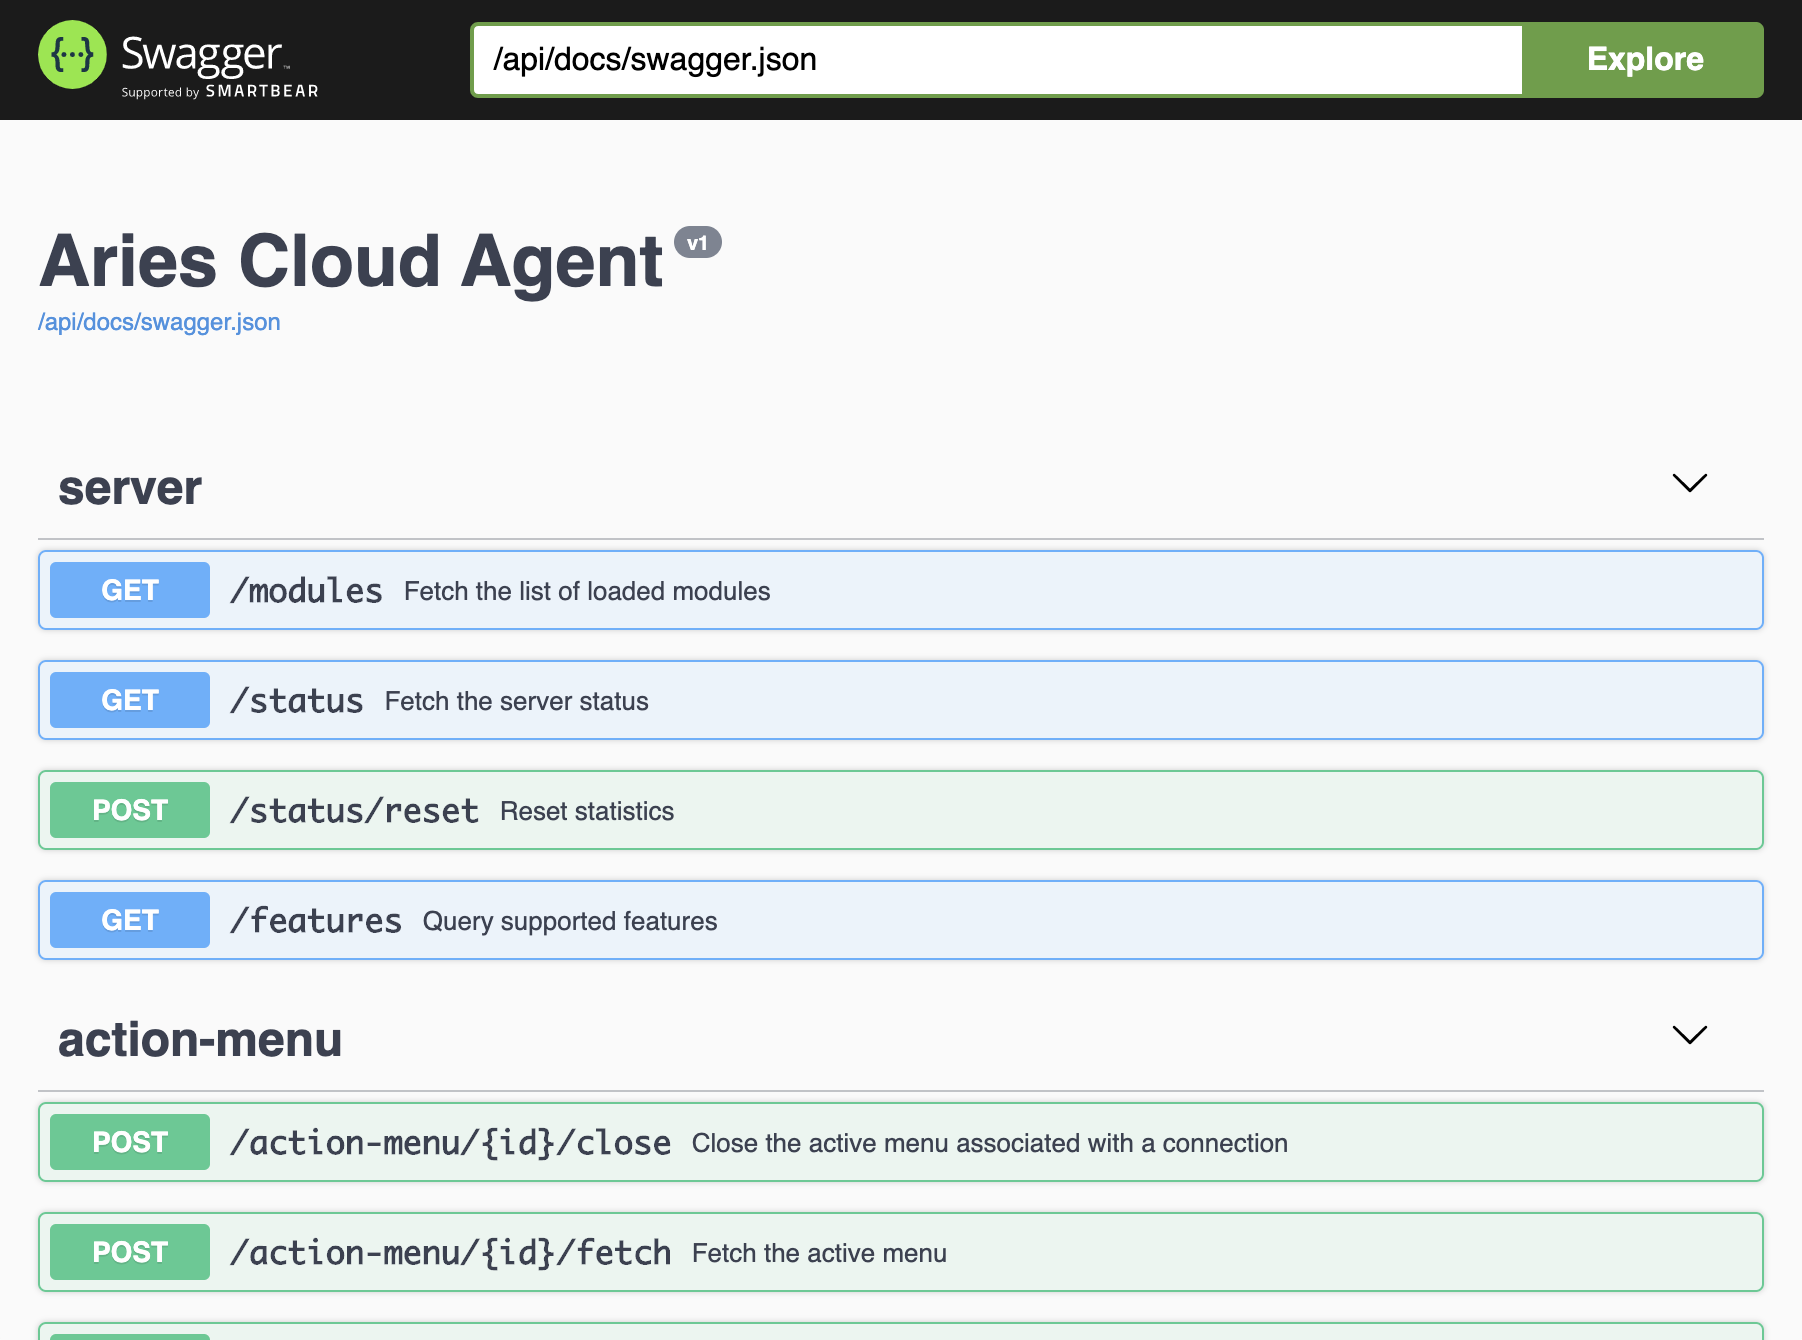
\includegraphics[scale=0.2]{adminApi.png}
\end{center}


\subsubsection{Aries Mobile Agent React-Native}
\noindent 
\begin{flushleft}
L'Aries Mobile Agent (ou Aries Bifold) est une application Open Source développée sur React Native 0.64.1 qui a pour but de regrouper les efforts de la communauté Aries Hyperledger orientée application mobile vers un projet centralisé, afin d'éviter la duplication du code et les similitudes entre les projets. Ce projet est aussi destiné à aider d'autres projets spécifiques voulant utiliser sur mobile les technologies de la fondation Aries Hyperledger sans avoir à redéfinir la complexité interne des agents Aries. Il est conçu pour permettre de démarrer rapidement un projet en ayant un agent Aries de base.\

Aries Mobile Agent est basé sur deux dépendances principales qui sont les suivantes :\\
\begin{itemize}

\item Aries Framework Javascript, un framework écrit en TypeScript pour la création d'agents Self Sovereign Identity. SSI est une approche visant l'idée que chacun contrôle ses propres données informatiques, ainsi qu'un contrôle de quand et comment elles sont fournies aux autres. De plus, lorsqu'une donnée est partagée, cela doit être fait avec fiabilité. Avec SSI, il n'y a pas d'autorité centrale détenant les données les transmettant à d'autres entités sur demande. Vous seul en êtes le possesseur. Ce framework a également pour but d'utiliser les services DIDComm qui visent à être en conformité avec les normes définies dans les RFC d'Aries.

\item Indy-sdk-react-Native : Il s’agit d’un Wrapper de Indy destiné à React Native. Son rôle est d’implémenter les fonctionnalités de Indy SDK afin qu’elles soient utilisables avec React Native. 

React Native est un framework d'applications mobiles Open Source conçu par Facebook. Il est utilisé pour développer des applications natives pour Android et iOS. Aries Bifold étant développé en React native 0.64.1, il cible l’API 29.0.3 d’Android, tandis que sur IOS il vise la version 10.0+ et il ne peut être utilisé que sur des appareils physiques pour le moment. La virtualisation est possible que sur Androidx86.

Aries Bifold nécessite un médiateur pour fonctionner. Le mobile Agent est configuré pour utiliser la médiation implicite. Il utilise par défaut Indicio Public Mediator, médiateur public de tests en ligne basé sur un Agent ACA-Py.
Un médiateur est un agent dont le but est de faire l'intermédiaire entre un Mobile Agent et un autre Agent (par exemple un Cloud Agent ACA-py), en relayant les messages transmis entre eux. Une connexion DIDComm est établie avec le médiateur.\
Ci-dessous nous pouvons voir le principe et fonctionnement d'un médiateur entre deux Agents Alice et Bob comme cela est présenté dans la norme "Aries RFC 0211: Coordinate Mediation Protocol"\footnote{\url{https://github.com/hyperledger/aries-rfcs/blob/main/features/0211-route-coordination/README.md
}} :\\

\begin{center}
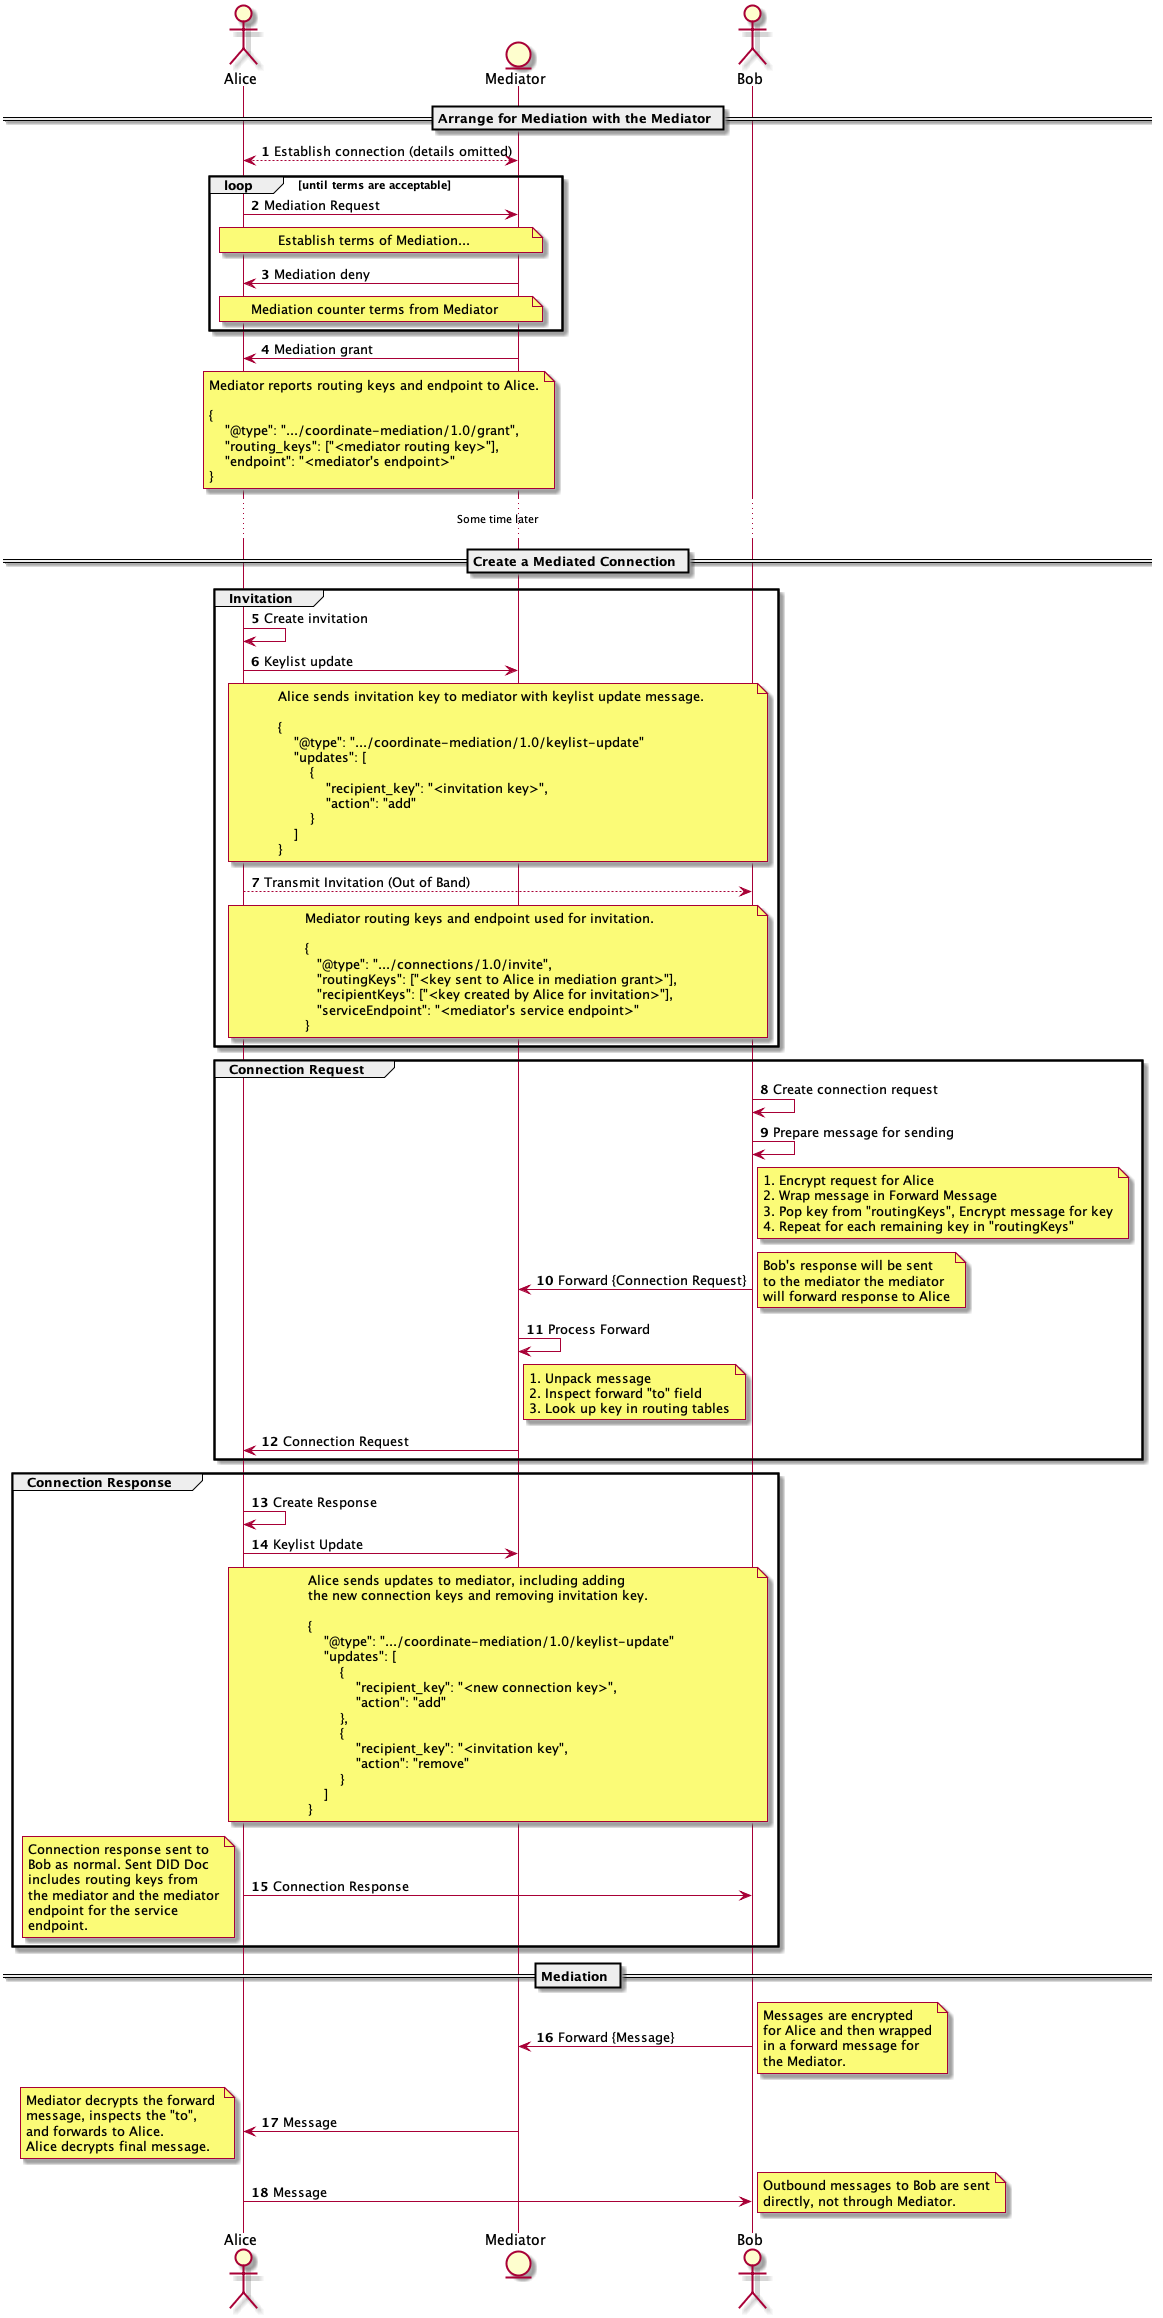
\includegraphics[scale=0.25]{mediator.png}
\end{center}

\end{itemize} 
\end{flushleft}


\subsection{QEMU}
\noindent 
\begin{flushleft}
QEMU est un logiciel libre  pouvant émuler un processeur ou une architecture différente. Il peut émuler un système ou juste le virtualiser, dépendant du système de l'hôte. QEMU peut exécuter différents systèmes d'exploitation et leurs applications de manière isolée sur une même machine physique ainsi que simuler les périphériques. \\
Dans notre projet nous nous sommes servis de QEMU pour émuler deux machines Debian et une machine Android
\end{flushleft}

\subsection{NEmu}
\noindent 
\begin{flushleft}
NEmu est un environnement permettant de mettre en place des réseaux virtuels. NEmu construit une topologie d'un réseau virtuel avec des Machines Virtuelles QEMU. NEmu met en place une API python rendant le travail plus facile. Il y a aussi la possibilité de simuler des dispositifs comme des routers ou des switchs pour mieux administrer le réseau. \\
Nous avons utilisé NEmu en combinaison avec QEMU pour construire un réseau de machines virtuelles.
\end{flushleft}

\section{Scénarios fonctionnels}
\noindent 
\begin{flushleft}
TODO
\end{flushleft}

\section{Architecture et implémentation}

\subsection{Réseau virtuel NEmu}
\noindent 
\begin{flushleft}
TODO
\end{flushleft}

\subsection{Mobile Agent du Client WireGuard}
\noindent 
\begin{flushleft}
TODO
\end{flushleft}

\subsection{Cloud Agent du Serveur WireGuard}
\noindent 
\begin{flushleft}
Le Serveur Wireguard est une machine qui hoste un service VPN Wireguard. Cette machine est une machine Debian. Dans cette machine il y a aussi un Agent Cloud. Cet Agent Cloud est capable de communiquae avec d'autres agents, notamment dans ce cas l'Agent du Serveur Blockchain et l'Agent du Client Wireguard. Il aura de différentes intéractions avec chacun des deux agents. \\
Avec l'Agent Server Blockchain il aura des interactions qui auront comme objectif la réception de Verifiable Credentials, ainsi que la vérification de ceux-ci. \\
Les échanges avec le Client Wireguard seront différents. En premier, il y aura un échange concernant les Verifiable Credentials - il faut que le Serveur Wireguard et le Client Wireguard s'échangent leur Verifiable Credentials/Presentations. Une fois les VC/P sont validés de chaque côté, les deux machines vont échanger leur clés publiques Wireguard pour pouvoir mettre en place un VPN. \\
Nous avons mis en place une interface graphique en python pour pouvoir gérer les différentes intéractions et événements.\\
TODO : AJOUTER IMAGE INTERFACE 
\end{flushleft}

\subsection{Cloud Agent du Serveur BlockChain}
\noindent 
\begin{flushleft}
Le Serveur Blockchain a différentes responsabilités. Dans le cas où on veut avoir notre propre réseau de noeuds Blockchain, le serveur Blockchain sera celui qui déploie ce réseau. Nous utilisons Von Network pour déployer les noeuds Blockchain. Nous avons aussi la possibilité de prendre comme référence un réseau de noeuds déjà éxistant. \\
Le Serveur Blockchain est donc celui qui est directemment rélié au réseau de noeuds Blockchain. Ce serveur enregistre les utilisateurs auprès de la Blockchain. Il se charge aussi de la délivrance de Verifiable Credentials et de la vérification de VC/VP. \\

\end{flushleft}

\section{Analyse du fonctionnement \& Tests}
\noindent 
\begin{flushleft}
TODO
\end{flushleft}

\section{Conclusion}
\noindent 
\begin{flushleft}
TODO
\end{flushleft}
\subsection{Limitations}
\noindent 
\begin{flushleft}
TODO
\end{flushleft}
\subsection{Extensions}
\noindent 
\begin{flushleft}
TODO
\end{flushleft}

\section{Bibliographie}
\noindent 
\begin{itemize}

\item WireGuard : \url{https://www.wireguard.com/} (consulté le 06/03/2022) 
\item Verifiable Credentials : \url{https://www.w3.org/TR/vc-data-model/} (consulté le 06/03/2022) 
\item Aries Cloud Agent : \url{https://github.com/hyperledger/aries-cloudagent-python} (consulté le 15/03/2022)
\item Aries Mobile Agent : \url{https://github.com/hyperledger/aries-mobile-agent-react-native/} (consulté le 15/03/2022)
\item Aries Framework Javascript : \url{https://github.com/hyperledger/aries-framework-javascript} (consulté le 15/03/2022)
\item React Native Indy SDK : \url{https://github.com/hyperledger/indy-sdk-react-native} (consulté le 15/03/2022)
\item QEMU : \url{https://www.qemu.org/} , \url{https://wiki.qemu.org/Main_Page} (consultés le 15/03/2022)
\item NEmu : \url{https://gitlab.com/v-a/nemu} (consulté le 15/03/2022)

\end{itemize}

\section{Annexe}
\noindent 
\begin{flushleft}
TODO
\end{flushleft}

\end{document}

%\begin{thebibliography}{}
%\bibitem[1]{1}
%https://www.wireguard.com/

%\end{thebibliography}
